\chapter{Implementierung und Anwendung}
In diesem Kapitel werden die Implementierung und Anwendung der entwickelten Pipelines für die jeweiligen Modelle beschrieben. Dabei wird auf die Implementierung der Modelle eingegangen und die Anwendung der Modelle auf die Datensätze beschrieben. Es soll deutlich werden, wie die Modelle implementiert wurden und wie sie in der Praxis v. a. in der Endanwendung angewendet werden können. Bei den hier aufgeführten Mechanismen handelt es sich um Eigenentwicklungen. Wurden schon bestehende Bibliotheken oder Frameworks verwendet, so wird dies explizit erwähnt bzw. in einer Fußnote darauf hingewiesen.

\section{Entwicklung der Verarbeitungspipeline}
In dieser Arbeit wurde der Entwicklungsprozess der Verarbeitungspipelines von dem CRISP-DM-Modell (Cross-Industry Standard Process for Data Mining) inspiriert. Das Vorgehen bei der Entwicklung aller Pipelines beginnt mit einem grundlegenden Verständnis der vorliegenden Daten, die aus Rechnungen aus dem unternehmensinternen Umfeld bestehen. Das Ziel besteht darin, Metadaten aus diesen Rechnungen zu extrahieren, um sie im JSON-Format für die Weiterverarbeitung in der Endanwendung aufzubereiten. Nachdem die Daten entsprechend aufbereitet wurden, kann das Modell trainiert werden. Die Modelle werden in der Endanwendung verwendet, um die Rechnungen zu klassifizieren und die Metadaten zu extrahieren. Anschließend erfolgt die Evaluation der jeweiligen Modelle. Bei zufriedenstellenden Ergebnissen kann das Modell in der Endanwendung eingesetzt werden. Den Trainingsdatensatz für das Finetuning bilden (zurzeit: Bei Bedarf anpassen) rund 850 größtenteils deutschsprachige Rechnungen aus dem Unternehmensumfeld. Die Rechnungen stammen aus verschiedenen Quellen, darunter E-Mails, PDFs und Scans. 
\begin{figure}[h!]
    \centering
    % Include the first image
    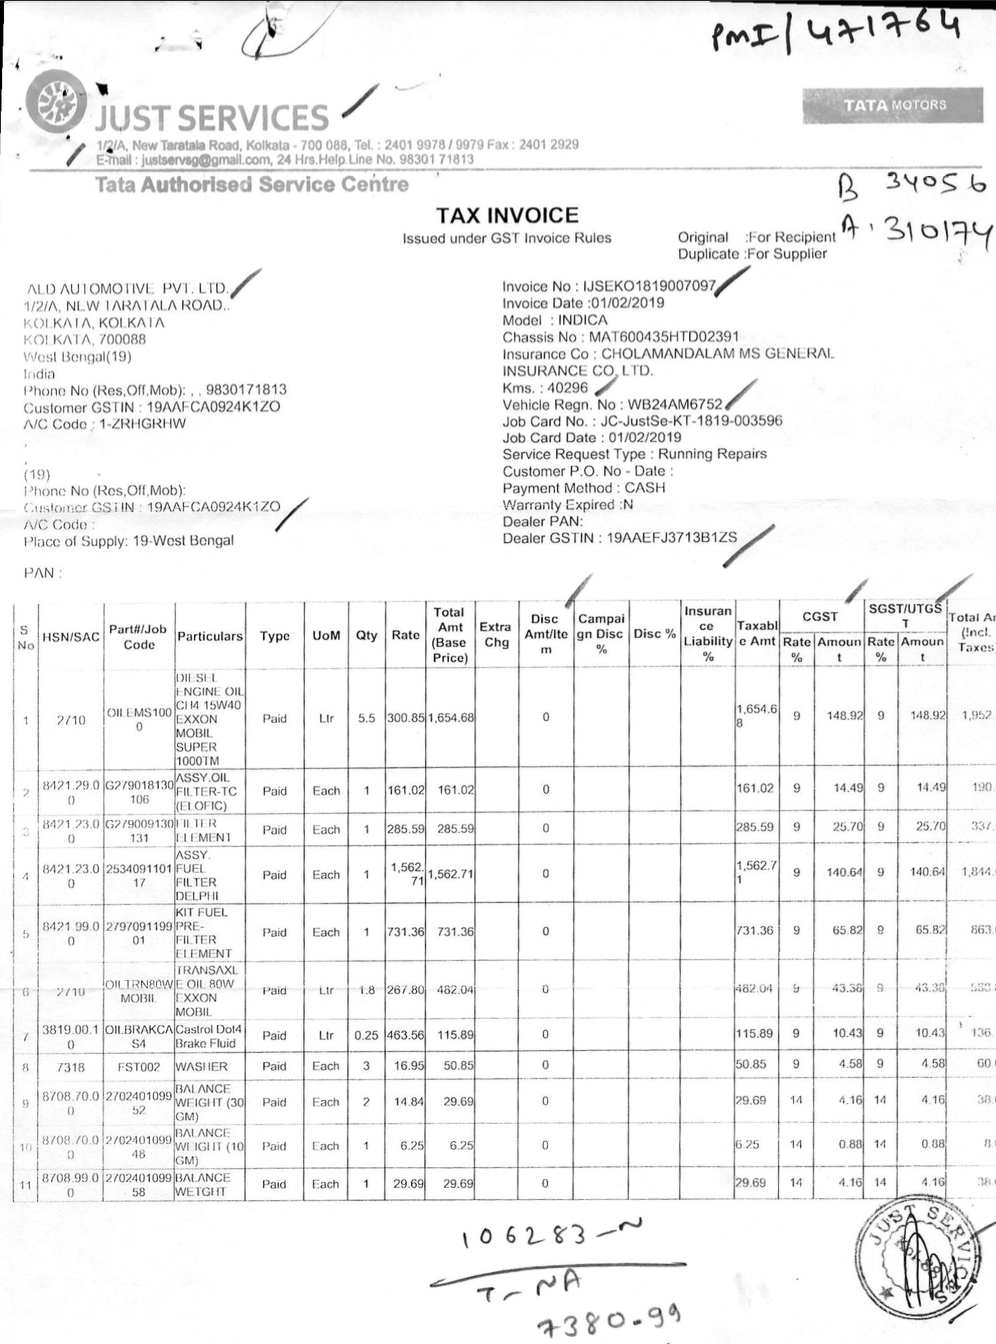
\includegraphics[width=0.45\textwidth]{graphics/bad_qual.png}
    \hfill % This adds space between the images
    % Include the second image
    \hfill % This adds space between the images
    % Include the third image
    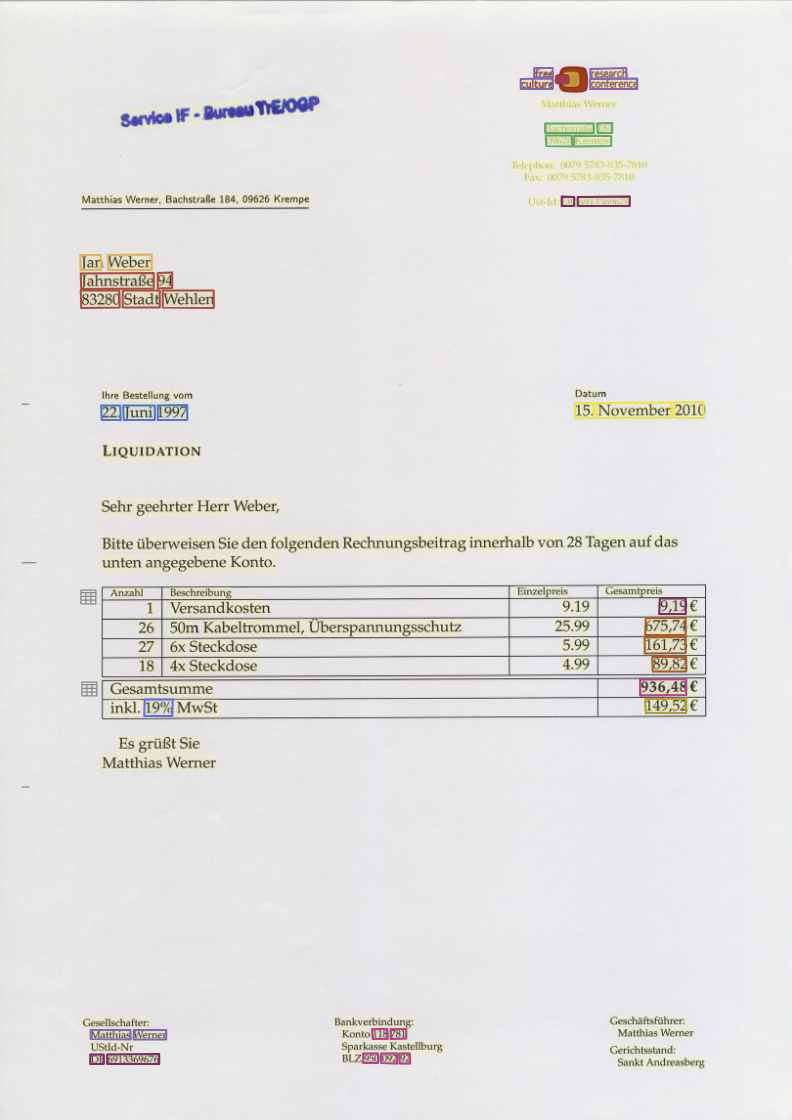
\includegraphics[width=0.45\textwidth]{graphics/doc_with_boc.png}
    \caption{Links: Beispiel für schlechte Qualität. Rechts: Beispiel für ein Dokument mit Bounding-Boxen und anderem Layout.}
    \label{fig:three_images}
  \end{figure}

Abbildung \ref{fig:three_images} zeigt, wie Layouts voneinander abweichen können. Links ist eine Rechnung mit einer vergleichsweise unübersichtlichen Tabelle zu sehen. Es gibt zudem viele händische Einträge. Die Rechnung in der Mitte ist deutlich übersichtlicher und strukturierter in Bezug auf das Layout. Die Rechnungen sind in unterschiedlichen Formaten und Layouts verfasst, um die Robustheit der Modelle zu testen. Die Rechnungen enthalten sowohl strukturierte als auch unstrukturierte Daten. Die strukturierten Daten umfassen beispielsweise Rechnungsnummer, Rechnungsdatum, Lieferdatum, Steuernummer, Umsatzsteuer-ID, IBAN, BIC, Gesamtbetrag, Steuersatz, Steuerbetrag, Netto- und Bruttobetrag. In Abb. \ref{fig:three_images} ist rechts ebenfalls eine Rechnung mit erkannten Daten zu sehen. Die farbigen Felder stellen die Bounding-Boxen der Felder dar. Die unstrukturierten Daten umfassen beispielsweise die Rechnungsadresse, die Lieferadresse, die Positionen, die Menge, die Einheit, den Preis und die Beschreibung. Die Rechnungen enthalten auch Logos, Werbung und andere Informationen, die nicht relevant sind. Diese müssen vor der Verarbeitung entfernt werden.

Der Prozess der Verarbeitungspipeline wird in Abb. \ref{fig:pipeline} dargestellt. Anders als üblicherweise empfohlen, erfolgt die Datenbereinigung in dieser Arbeit erst nach der ersten Verarbeitung. \footcites[Vgl. dazu ausführlich][]{wirth_crisp-dm_2000} Die initiale Phase umfasst die Annotation der Daten. Aufgrund begrenzter Ressourcen wird hierfür das Azure Document Intelligence Studio mit einem Custom Model genutzt, das speziell darauf ausgelegt ist, die Rechnungen zu labeln. Azure wird insbesondere wegen der begrenzten zeitlichen Ressourcen eingesetzt, da nicht genügend Zeit zur Verfügung steht, um die Daten händisch zu annotieren. Die Entscheidung für Azure und die sich daraus ergebenden Implikationen werden in einem späteren Kapitel diskutiert. Azure verwendet als OCR-Engine die proprietäre Microsoft Read OCR. Diese ist u. a. mit KI-Modellen verbessert worden, um bessere Ergebnisse im Bereich des \ac{Vrdu} zu erzielen. Ein Beispiel einer vollständig gelabelten Datei kann Anhang x entnommen werden. Es wird unterschieden zwischen Labeling-Verfahren für OCR-abhängige Modelle und solche, die unabhängig davon agieren. Für die unabhängigen Modelle werden keine Bounding-Boxen inkludiert. Bei Bounding-Boxen handelt es sich um vier Koordinaten in einem Dokument, die ein Rechteck um ein Wort oder eine Zeile bilden. Diese Bounding-Boxen sind notwendig, um die Position der Wörter im Dokument zu bestimmen (s. als Beispiel Abb. \ref{fig:three_images}). 

\begin{figure}[]
    \centering
    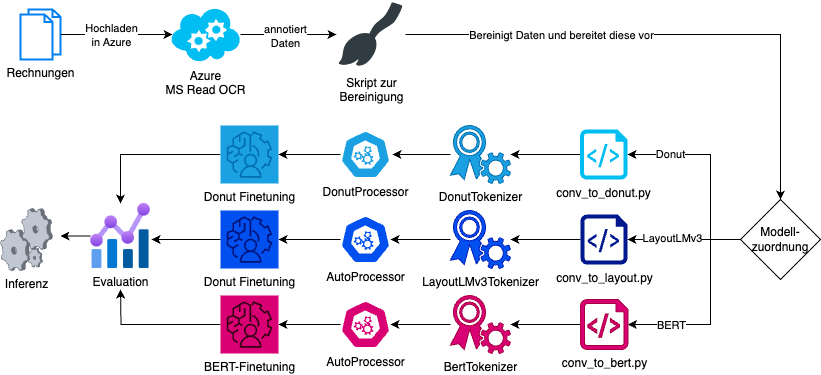
\includegraphics[width=160mm]{graphics/verarbeitungspipeline.png}
    \caption[Finetuning-Pipeline]{Finetuning-Pipeline}
    \label{fig:pipeline}
\end{figure}

Nach der Annotation werden aus dem Datensatz alle Dokumente, die keine Rechnungen sind oder einzelne Seiten dieser entfernt. Dies könnte zum Beispiel die letzten Seiten einer Rechnung betreffen, die Werbeslogans oder Verweise auf den Webshop enthalten. Die Aufbereitung der Daten unterscheidet sich je nach Modell. Während für LayoutLMv3 die Daten aus JSON in Listen umgewandelt und Bounding-Boxen normalisiert werden müssen, können die Daten für Donut im JSON-Format verbleiben. Ein Beispielhaftes JSON, welches  für das Training von aufbereitet wurde, Donut kann Abbildung x entnommen werden. In der Inferenz von Donut wird erwartet, dass die Informationen in diesem JSON-Format wieder ausgegeben werden.

\begin{figure}[]
    \centering
    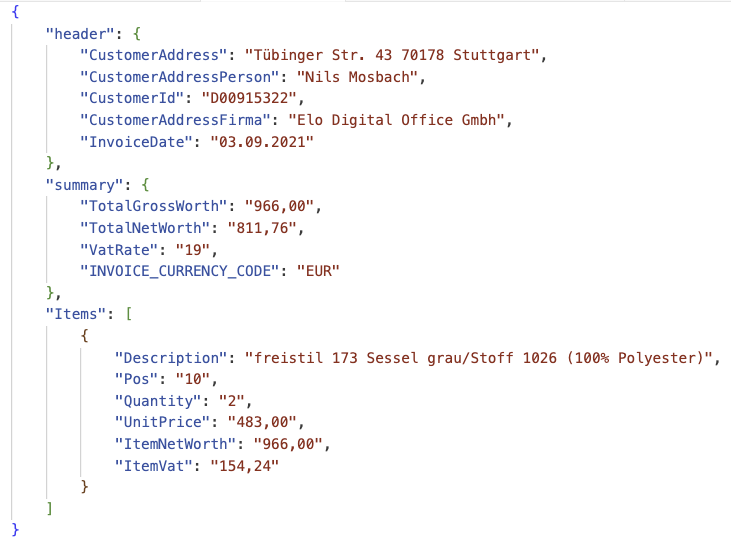
\includegraphics[width=100mm]{graphics/json-example.png}
    \caption[Beispielhaftes JSON]{Beispielhaftes JSON}
    \label{fig:json_example}
\end{figure}

Allerdings erfordert dies ein Mapping zwischen jedem JSON und dem zugehörigen Bild der Rechnung im Verzeichnis. Die nachfolgende Tokenisierung wird für alle drei Modelle mit modellspezifischen Tokenizern durchgeführt. Für die Erzeugung der Embeddings wird ebenfalls modellspezifisch vorgegangen, wobei jeder Modelltyp einen spezifischen Processor benötigt. Beim Processor handelt es sich um eine Klasse, die die Daten in ein für das Modell verständliches Format von Token Embeddings umwandelt.

Nach der Erzeugung der Embeddings durchlaufen die Modelle das Feintuning. Abgeschlossen wird dieser Prozess durch eine Evaluation mit 40 Rechnungen. In der abschließenden Inferenzphase wird das Modell mit einer Rechnung gefüttert, und die extrahierten Daten werden in einem strukturierten Format (in diesem Fall JSON) ausgegeben, was den gesamten Prozess der Verarbeitungspipeline abschließt.

\section{Besonderheiten von Donut in der Implementierung}
Das folgende Kapitel soll einen Überblick über die Gemeinsamkeiten und Unterschiede der Implementierung von Donut im Vergleich zu den anderen Modellen geben. Aus Gründen der Anschaulichkeit wird hierbei LayoutLMv3 als Vergleich verwendet. Die meisten Aspekte treffen jedoch auch auf das Modell BERT zu.

Bei der Gegenüberstellung der Finetuning-Pipelines für Donut und LayoutLMv3 fällt auf, dass die beiden Ansätze sowohl Gemeinsamkeiten als auch Unterschiede aufweisen, die jeweils für die spezifischen Anforderungen ihrer Modelle optimiert sind.

Es zeigen sich folgende Gemeinsamkeiten in der Implementierung: Beide Modelle verwendet spezialisierte Prozessoren (DonutProcessor für Donut und LayoutLMv3Processor für LayoutLMv3), um Bilder und Textdaten entsprechend vorzubereiten. Zusätzllich muss bei beiden Modellen auf die gründliche Bereinigung und Vorbereitung der Trainingsdaten gelegt werden. Bereits ein fehlerhaftes Dokument in den Trainingsdaten kann zu einer schlechten Performance der Modelle führen oder das Finetuning als Ganzes verhindern. Beide Modelle verwenden individuelle Trainingsdatensätze, die speziell darauf ausgerichtet sind, die für das jeweilige Modell erforderlichen Informationen zu verarbeiten und bereitzustellen. Die Eingangsdaten sind für alle Modelle dieselben. Sie unterscheiden sich lediglich in ihrer Aufbereitung. Die Trainingskonfiguration ist für beide Modelle dieselbe. Dazu gehören beispielsweise die Anzahl an Trainingsepochen, die Anzahl an Validierungen pro Epoche und die Trainingsschrittgröße. In einem späteren Kapitel wird im Detail auf die Trainingskonfiguration bzw. die Hyperparameter eingegangen. Für die grundlegende Gegenüberstellung bleiben sie jedoch gleich.

In der Verarbeitungspipeline für Donut werden dennoch mehr Unterschiede zu LayoutLMv3 als Gemeinsamkeiten deutlich. Den ersten maßgeblichen Unterschied bildet der Zugriff auf die Datensätze. Für die Verarbeitungspipeline von Donut war es notwendig, die Daten in einem speziellen Format zu speichern, das für das Modell geeignet ist. Daher wurde eine eigens entwickelte Dataset-Klasse(DonutDataset) verwendet, die speziell für die Verarbeitung und das Handling von Bild- und Textdaten entwickeltet wurde. Sie hat den Vorteil, dass die annotierten Daten im JSON Format nicht weiter transformiert werden müssen. Es braucht lediglich ein Mapping zwischen dem Bild, welches annotiert wurde und dem zugehörigen JSON. LayoutLMv3 greift auf bestehende Funktionalitäten der HuggingFace dataset-Bibliothek zurück. Hier müssen die Daten viel aufwendiger in eine Reihe von Listen bestehden aus \emph{Tokens, Bounding-Boxen, Labeln und Bildern} umgewandelt werden. Bounding-Boxen müssen zusätzlich normalisiert werden, was den Rechenaufwand nochmals linear erhöht. Bei Donut wird zudem auf eine differenzierte Annotation der Daten Wert gelegt, wobei layoutbasierte Informationen wie die zuvor genannten Bounding-Boxen nicht inkludiert werden. Dies führt zu einer einfacheren und schnelleren Annotation der Daten. Ein weiterer Unterschied besteht in der Tokenisierung und Eingabeverarbeitung. Die in dieser Arbeit entwickelte Donut-Pipeline umfasst spezielle Schritte zur Tokenisierung und Eingabeverarbeitung, die an das Design und die Anforderungen des Donut-Modells angepasst sind. LayoutLMv3 nutzt hingegen den AutoProcessor für eine automatisierte Verarbeitung, basierend auf dem Modellcheckpoint. Der AutoProcessor lädt für das jeweilige Modell den benötigten Processor automatisch. Schlussendlich zeigen sich bedeutende Unterschiede im Trainigns- und Evaluationssetup. Während Donut spezifische Klassen und Funktionen für das Training und die Evaluation implementiert, einschließlich angepasster Callbacks und einer umfangreichen Konfiguration, folgt LayoutLMv3 einem standardisierten Trainings- und Evaluationsprozess, der auf den HuggingFace-Trainings- und Evaluationsfunktionen basiert.

Die im Rahmen dieser Arbeit entwickelte Donut-Pipeline zeichnet sich v. a. durch zwei besondere Merkmale aus:
\begin{itemize}
    \item \textbf{Flexibilität in der Datenverarbeitung:} Die Donut-Pipeline zeichnet sich durch eine hohe Flexibilität bei der Aufbereitung und Anpassung der Trainingsdaten aus, um die Anforderungen des Modells optimal zu erfüllen.
    \item \textbf{Erweiterte Tokenisierung und Spezialtokens:} Die Donut-Pipeline beinhaltet spezielle Schritte zur Erweiterung der Tokenisierung und zur Integration von Spezialtokens, die für das Training und die Generierung von Vorhersagen entscheidend sind.
\end{itemize}

Insgesamt zeigt der Vergleich, dass beide Pipelines spezifisch für die Bedürfnisse und die Architektur der jeweiligen Modelle entwickelt wurden, mit besonderem Fokus auf die Optimierung der Datenvorbereitung, des Trainings und der Evaluation. Die Donut-Pipeline sticht durch ihre spezialisierte Herangehensweise und Anpassungsfähigkeit hervor, während die LayoutLMv3-Pipeline auf bewährte Methoden und Werkzeuge setzt, um eine effiziente Modellanpassung zu ermöglichen. Tabellen \ref{tab:donut_layoutlmv3_comparison} stellt die Unterschiede und Gemeinsamkeiten der Finetuning-Pipelines von Donut und LayoutLMv3 übersichtlich gegenüber.

Es ist wichtig hervorzuheben, dass es bedeutend Aufwendiger ist, eine Pipeline für Donut zu entwickeln, als für LayoutLMv3 oder BERT. Die beiden Referenzmodelle sind deutlich robuster im Hinblick auf das Preprocessing und die Eingabedaten. Dies kann dadurch erklärt werden, dass es sich bei BERT um ein bereits sehr etabliertes Modell handelt und LayoutLMv3 zusätzlich von Microsoft entwickelt wurde und daher auf eine Vielzahl von Ressourcen zurückgreifen kann. Donut hingegen ist ein relativ neues Modell, das noch nicht so weit verbreitet ist. Es handelt sich um ein offenes, nicht proprietäres Modell, das von einer kleinen Gruppe von Entwicklern entwickelt wurde. Daher ist es notwendig, eine spezialisierte Pipeline zu entwickeln, um das Modell optimal zu nutzen.

\begin{table}[ht]
    \centering
    \begin{tabularx}{\textwidth}{@{}lXX@{}}
    \toprule
    \textbf{Aspekt} & \textbf{Donut} & \textbf{LayoutLMv3} \\
    \midrule
    Spezialisierte Prozessoren & Verwendet DonutProcessor & Verwendet LayoutLMv3Processor \\
    Datenbereinigung & Hohe Flexibilität bei der Datenvorbereitung & Erfordert umfangreiche Datenbereinigung und -vorbereitung \\
    Trainingsdatensätze & Verwendet eine speziell entwickelte Dataset-Klasse (DonutDataset) & Greift auf bestehende Funktionalitäten von Hugging Face zurück \\
    Annotation der Daten & Differenzierte Annotation ohne Bounding Boxes für layoutbasierte Informationen & Verwendet detaillierte Annotationen inklusive Bounding Boxes \\
    Tokenisierung & Spezielle Schritte zur Tokenisierung und Eingabeverarbeitung, angepasst an das Modell & Nutzt den AutoProcessor für automatisierte Verarbeitung \\
    Trainings- und Evaluationssetup & Implementiert spezifische Klassen und Funktionen für das Training und die Evaluation & Folgt einem standardisierten Trainings- und Evaluationsprozess \\
    \bottomrule
    \end{tabularx}
    \caption{Vergleich der Finetuning-Pipelines von Donut und LayoutLMv3}
    \label{tab:donut_layoutlmv3_comparison}
\end{table}
    

\section{Diskussion der Implementierung}
Eine umfassende Diskussion und kritische Betrachtung der vorliegenden Bachelorarbeit erfolgt in Kapitel 6. Dennoch soll der folgende Abschnitt eine kruze Diskussion der Implementierung der Modelle und der Verarbeitungspipelines bieten. Damit sollen einige Entscheidungen erläutert werden und die Gründe für die gewählten Vorgehensweisen dargelegt werden.

Die im vorherigen Abschnitt erläuterten Besonderheiten der Donut-Pipeline treffen nicht zwingend auf jede Donut-Pipeline zu. Die Implementierung der Donut-Pipeline in dieser Arbeit wurde speziell auf die Anforderungen des Modells und die verfügbaren Ressourcen zugeschnitten. Des weiteren erfolgte die Implementierung unter der Annahme, das Modell in der Endanwendung bei ausreichend guten Ergebnissen einzusetzen. Daher wurde hier der Fokus auf die Optimierung von Donut gelegt. Hiermit lassen sich auch die Flexibilität der Datenverarbeitung und die erweiterte Tokenisierung und Spezialtokens erklären. Die Implementierung der LayoutLMv3- und BERT-Pipeline hingegen erfolgte unter der Annahme, dass die Modelle nur als Vergleichsmodelle dienen soll. Daher wurde hier auf bewährte Methoden und Werkzeuge zurückgegriffen, um eine effiziente Modellanpassung zu ermöglichen. Die Implementierung der BERT-Pipeline erfolgte unter der Annahme, dass das Modell als Backup-Modell für Donut dienen soll. Daher wurde hier auf eine effiziente Implementierung geachtet, die eine schnelle Anpassung und Integration in die Endanwendung ermöglicht. Die im vorgegangen Abschnitt implizierten Vorteile können zu großen Teilen auch auf die anderen Pipelines übertragen werden. Da die Vergleichsmodelle jedoch nur zu Forschungszwecken eingesetzt werden, wurde hier auf eine spezialisierte Implementierung, d. h. auf eine, die unter Umständen in der Endanwendung verwendet werden könnte, verzichtet.

Eine Schwachstelle der Implementierung ist die Verwendung vom Azure Docuement Intelligence Studio für die Annotation der Daten. Azure bietet zwar eine schnelle und effiziente Möglichkeit, die Daten zu annotieren, jedoch ist das Format stellenweise nicht passend für die Weiterverarbeitung in Transformern angepasst. Für LayoutLMv3 gibt Azure auch Bounding-Boxen bei der Annotation zurück. Diese sind jedoch in Zoll formatiert. Daher ist noch die Transformation aller Größen in Pixeln notwendig. Dies führt zu einem erhöhten Rechenaufwand und einer längeren Verarbeitungszeit. Ein weiterer Nachteil ist die Abhängigkeit von Azure. Sollte Azure nicht verfügbar sein, wäre die automatisierte Annotation der Daten mittels vortrainierter Modelle nicht möglich. Diese Form der Annotation nutzt maschinelle Lernmodelle, die auf der Azure-Plattform gehostet werden, um Textelemente in den Dokumenten zu erkennen und entsprechend zu klassifizieren. Der Einsatz solcher Modelle verursacht Rechenaufwand, da jede Annotation eine Vorhersage durch das Modell erfordert, welches rechenintensive Prozesse wie das Laden des Modells, die Verarbeitung der Eingabedaten und die Ausführung der inferentiellen Algorithmen umfasst. Sollte Azure nicht verfügbar sein, wäre die automatisierte Annotation der Daten mittels vortrainierter Modelle nicht möglich. Diese Form der Annotation nutzt maschinelle Lernmodelle, die auf der Azure-Plattform gehostet werden, um Textelemente in den Dokumenten zu erkennen und entsprechend zu klassifizieren. Der Einsatz solcher Modelle verursacht Rechenaufwand, da jede Annotation eine Vorhersage durch das Modell erfordert, welches rechenintensive Prozesse wie das Laden des Modells, die Verarbeitung der Eingabedaten und die Ausführung der inferentiellen Algorithmen umfasst.
